%!TEX root = ../../report.tex
\subsection{Logical View}

\copied{Logical view : The logical view is concerned with the functionality that the system provides to end-users. UML Diagrams used to represent the logical view include Class diagram, Communication diagram, Sequence diagram.[2]}
{from wikipedia\\\url{https://en.wikipedia.org/wiki/4\%2B1_architectural_view_model}}

The logical view shows the structural elements, key abstractions and mechanisms that are needed to realize the SFM. First an overview of the different components is provided. After that the components are decomposed and more details of the different layers are provided.

% This view shows the structural elements, key abstractions and mechanisms that are used within SFM to realize the systemics functionality. At first an overview of the components is provided. After that the main components are decomposed and desired in term of responsibilities and interfaces. In the end, the variability guide mentions parts of the software, which clarification is deferred until development/design phase.



%Used algorithms?:
%	hidden markov model with k means (unsupervised learning)
%	Singular Spectrum Analysis (SSA) for locations with tides?
%	“limit checking”
%	
%	Gauss-Markov
%	Something with correlation? https://en.wikipedia.org/wiki/Cross-correlation? Thesis zecht te kijken naar:
%	[74] Logan, D., Mathew, J. Using the Correlation Dimension for Vibration Fault
%Diagnosis of Rolling Element Bearing – I. Basic Concepts, Mechanical Systems and
%Signal Processing, Vol. 10, No. 3, pp. 241-250, (1996)
%[75] Logan, D., Mathew, J. Using the Correlation Dimension for Vibration Fault
%Diagnosis of Rolling Element Bearing – II. Selection of Experimental Parameters,
%Mechanical Systems and Signal Processing, Vol. 10, No. 3, pp. 251-264, (1996)

\subsubsection*{Layer pattern}
The software architecture of SMF is separated into three different layers. This layering is done according to the layering Martin Fowler proposes for enterprise applications \cite{Fowler:2002:PEA:579257,Fowler:web:servicelayer}.
Layering the software provides a more flexible architecture that allows modifications of layers having to alter the other layers.\\
The different software layers of SMF are listed below. Each of these layers will be discussed in more detail after the figure.

\begin{description}
	\item \textbf{Service layer} This layer provides services to external systems and coordinates the incomming calls to the domain layer.
	\item \textbf{Domain layer} The domain layer holds the core components for processing data and warning users.
	\item \textbf{Data source layer} This layer stores all relevant data that is needed or produced by the system. 
\end{description}

\clearpage
\begin{figure}[H]
	%\centering
	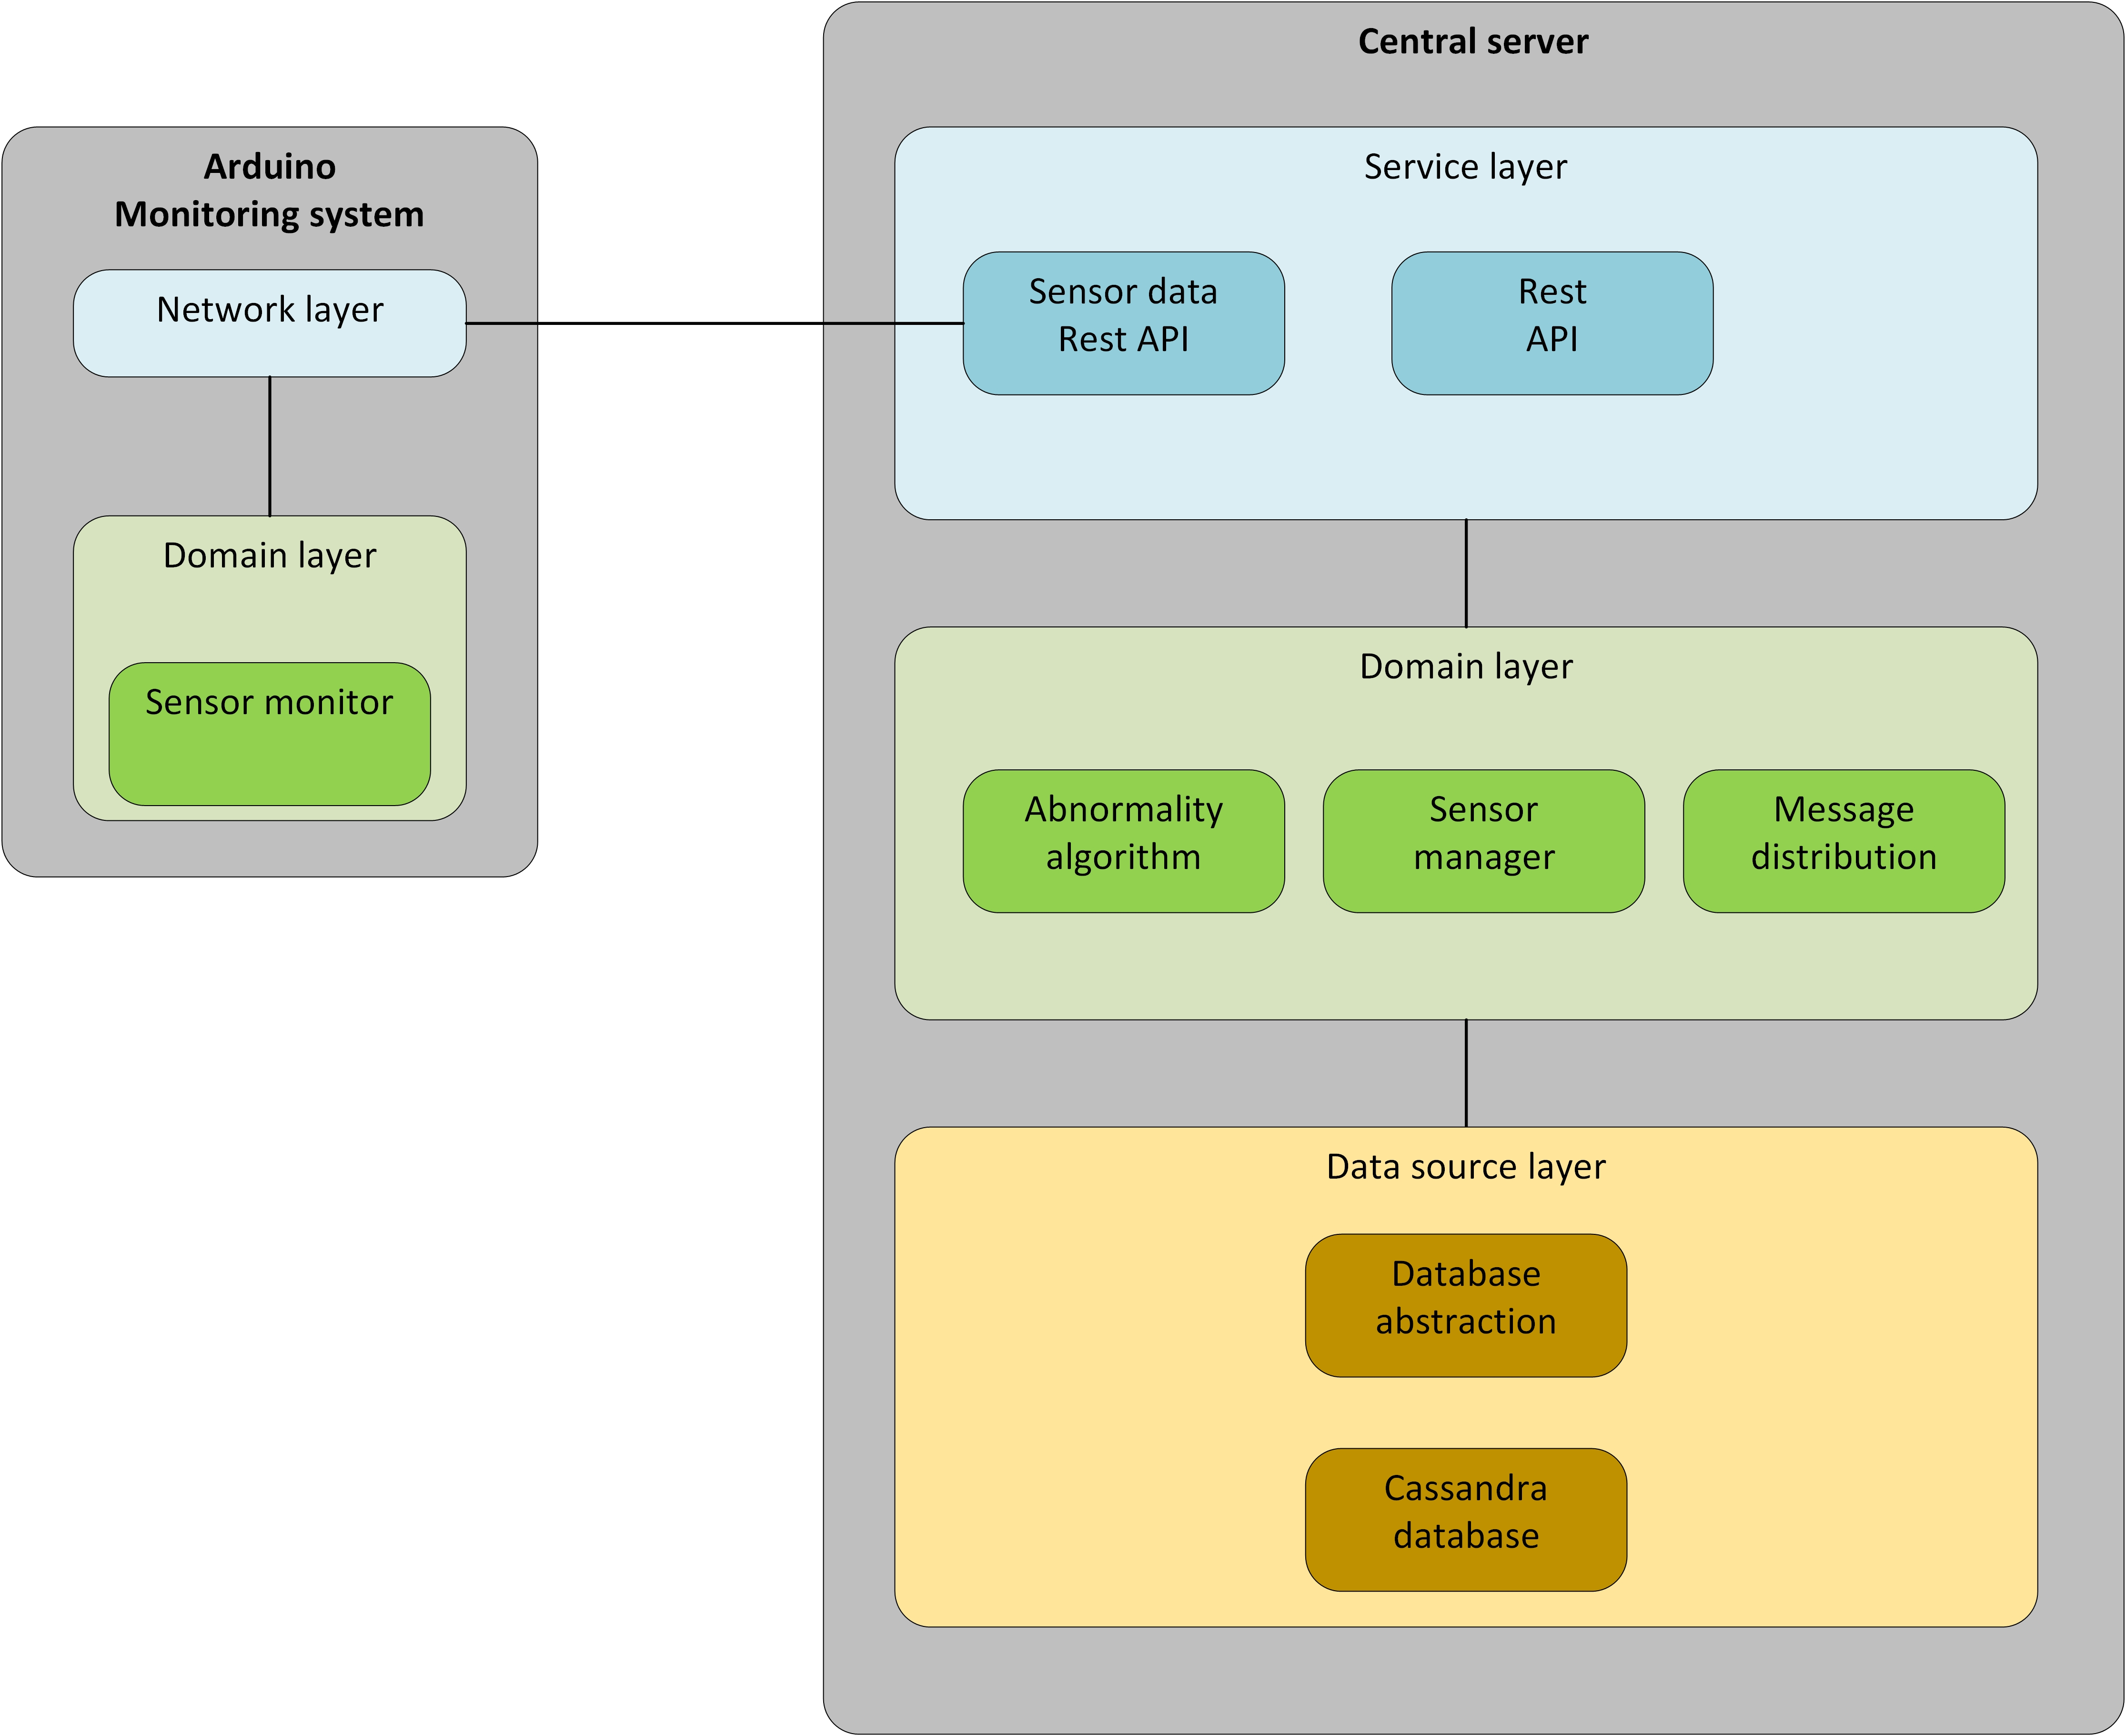
\includegraphics[keepaspectratio=true,width=0.9\textwidth]{{\viewimages/layers}.jpg}
	\caption{Layers of the software}
	\label{fig:layers}
\end{figure}

\subsubsection*{Service layer}
The Service layer pattern \cite{Fowler:2002:PEA:579257} is used as domain logic pattern. In this pattern, the service layer provides a set of operations that can be executed in the application. The service layer serves and coordinates the calls to these provides operation. The application logic in the domain layer is then separated from how it is called and how it should respond.\\
The main functionality of this layer consists of:
\begin{itemize}
	\item Providing a REST server the arduino monitoring units can send their raw sensor data to
	\item Providing a REST server the third parties can use to receive flood data
	\item Distribute warning messages
\end{itemize}

The class diagram for this layer is shown in figure \ref{fig:service1}

\begin{figure}[H]
	\centering
	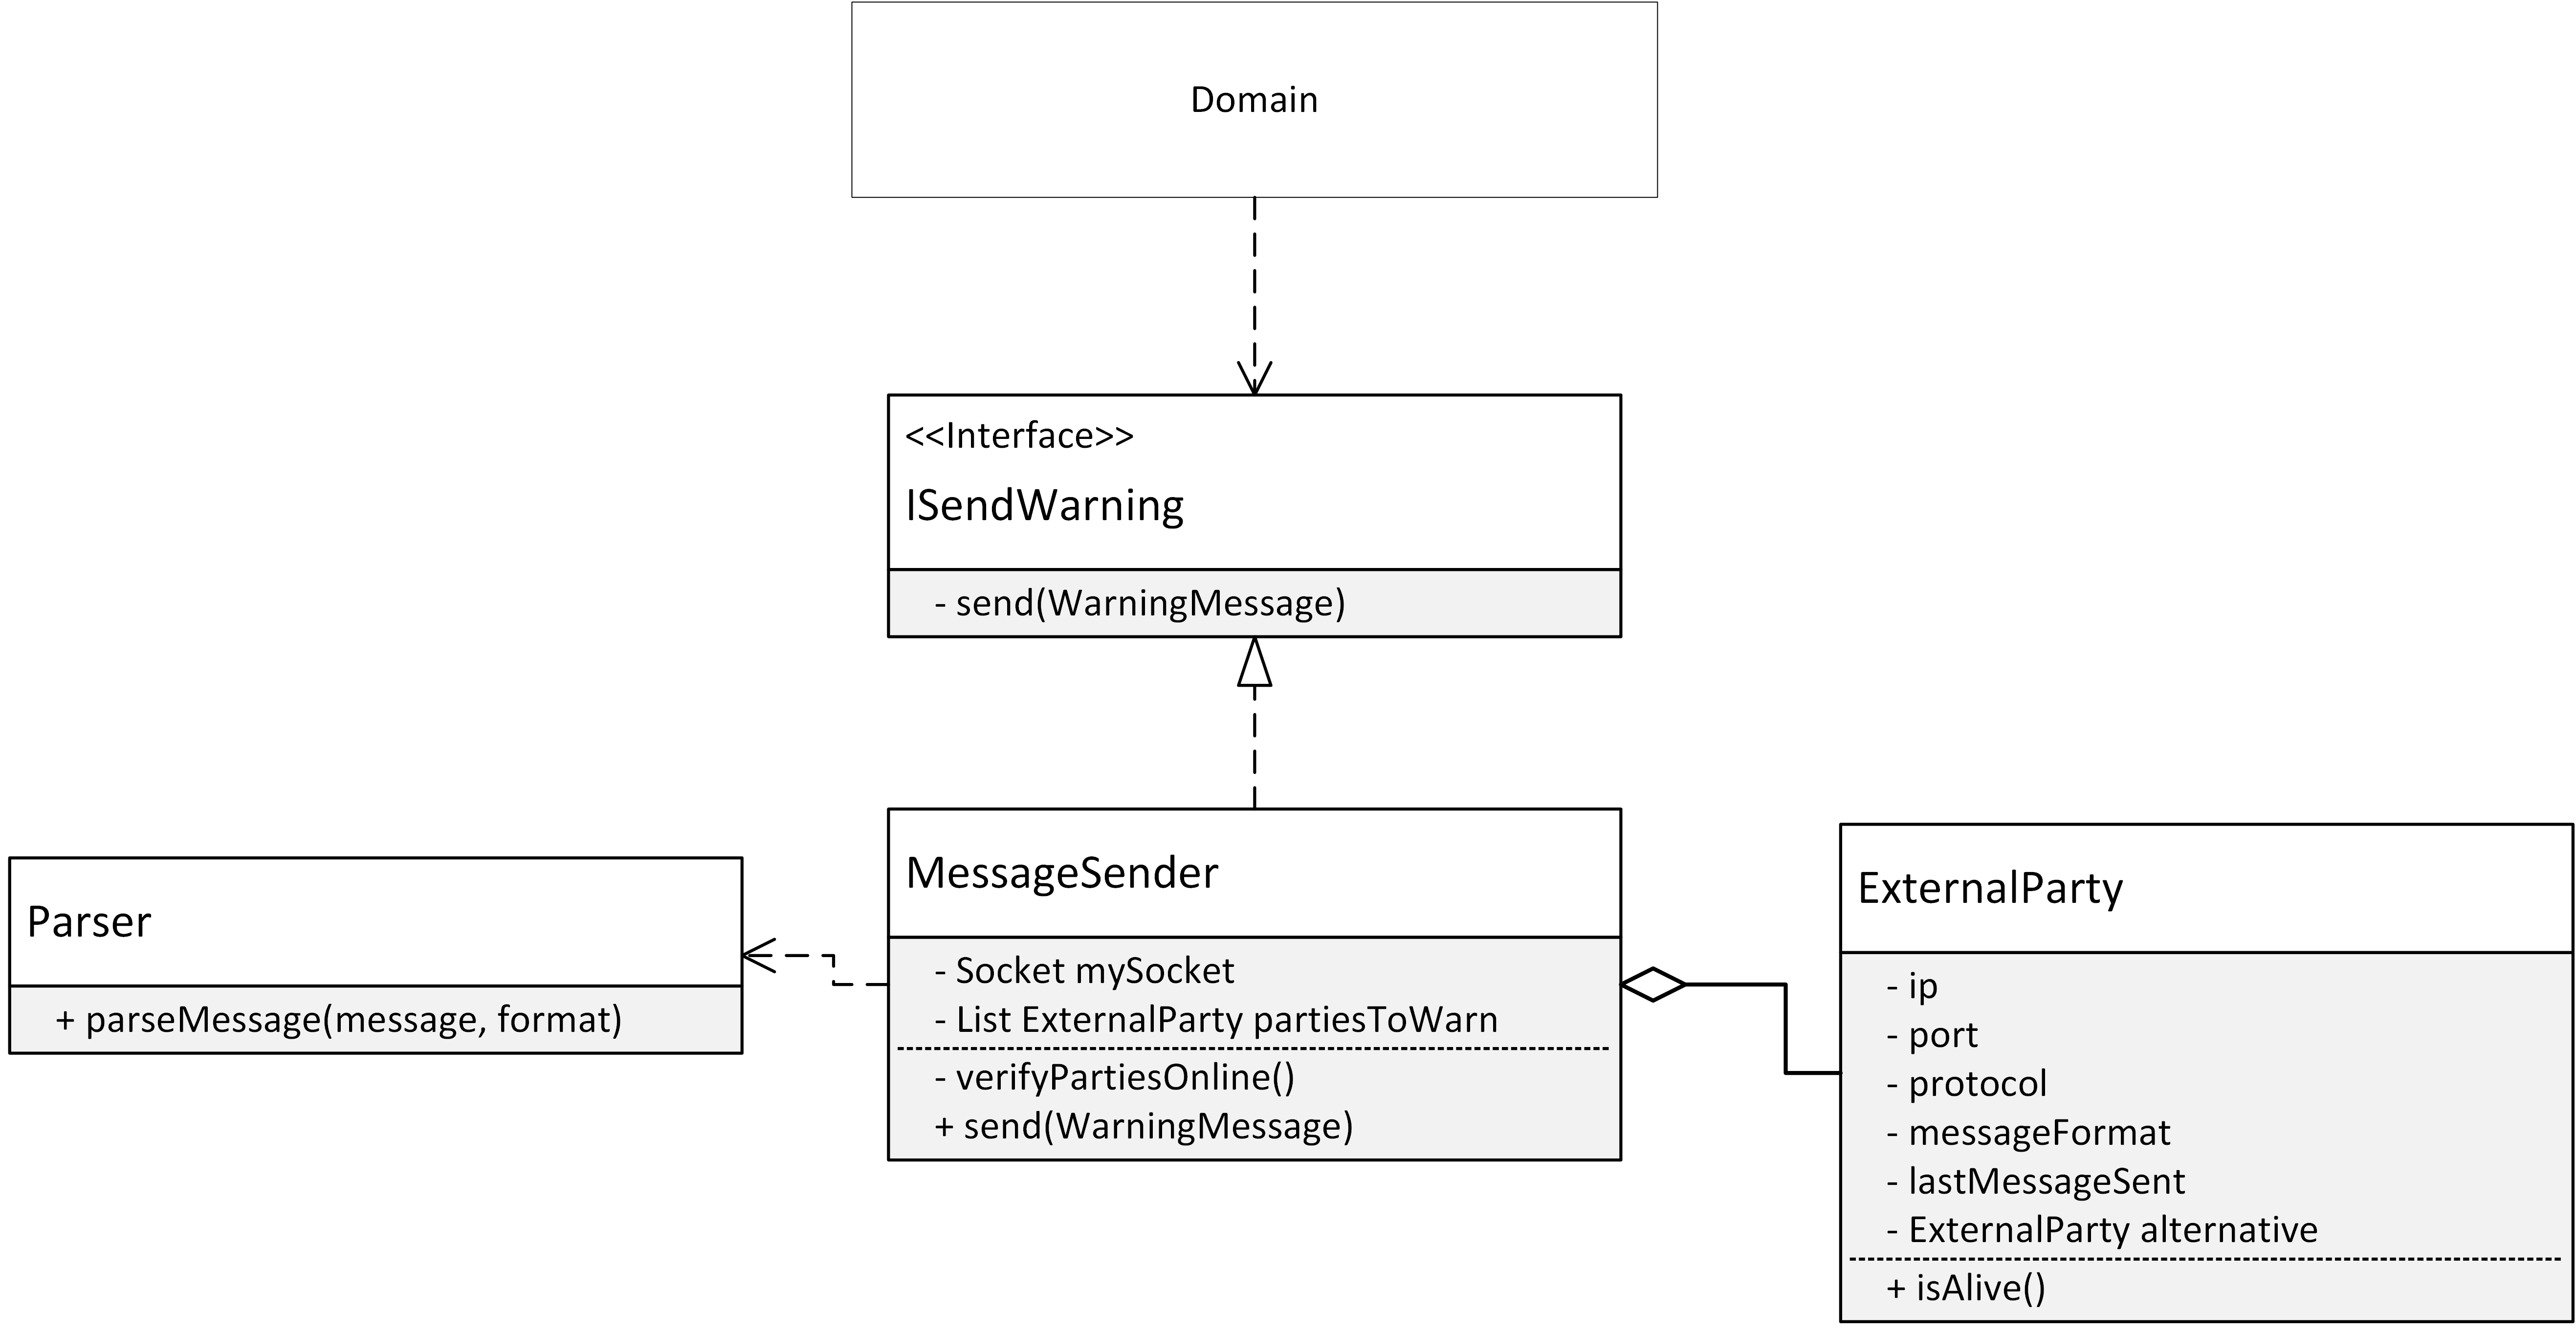
\includegraphics[keepaspectratio=true,width=1.0\textwidth]{{\viewimages/service1}.jpg}
	\caption{Class diagram of service layer}
	\label{fig:service1}
\end{figure}

The sensors periodically send their sensor data to the central server. This is illustrated in figure \ref{fig:sensorseq}
\begin{figure}[H]
	%\centering
	\includegraphics[keepaspectratio=true,width=0.9\textwidth]{{\viewimages/sequence_sensor}.png}
	\caption{Sequence diagram of the client pushing the sensor data}
	\label{fig:sensorseq}
\end{figure}

\textbf{\textsc{URL}}
\begin{lstlisting}
/monitor/{monitorid}/sensorvalues
\end{lstlisting}

\textbf{\textsc{REQUEST HEADERS}}
\begin{lstlisting}
Content-Type: application/json
Authorization: <<Hash>>
\end{lstlisting}

\textbf{\textsc{REQUEST BODY}}
\begin{lstlisting}
[
	{
		sensor: "<<sensorid>>",
		value: "<<value>>"
	},
	{
		sensor: "<<sensorid2>>",
		value: "<<value2>>"
	},
	...
]
\end{lstlisting}


%TODO (should push/pull be a decision?)
%TODO (HMAC should be a decision, could also use other hashes and verification)

The arduino system only pushes the data to the server. This push model reduces the load of the arduino systems because there are no incoming requests. This way, the arduino also doesn't have to store or manage any data, which also means the arduino doesn't need security measurements to secure this data.\\
The server does however need to verify that the messages it receives from the arduino monitoring systems are in fact send by our arduino systems. Otherwise a hacker could send sensor messages too, which would jeopardize the entire flood warning system.The downside to having the arduino systems push the data, is that data will be received by the server was not needed or wanted. Defect sensors data will still be send. \\
%http://rc3.org/2011/12/02/using-hmac-to-authenticate-web-service-requests/
% HMAC suggested by microsoft: https://msdn.microsoft.com/en-us/library/dd203052.aspx
 
The message security is done by using a hash based message authentication code (HMAC) using SHA-256 as the hashing algorithm. Upon receiving the messages, the service layer verifies the message before further processing the message.\\
The sequence of actions for obtaining information from SFM is shown below in figure \ref{thirdpartyseq}.
\begin{figure}[H]
	%\centering
	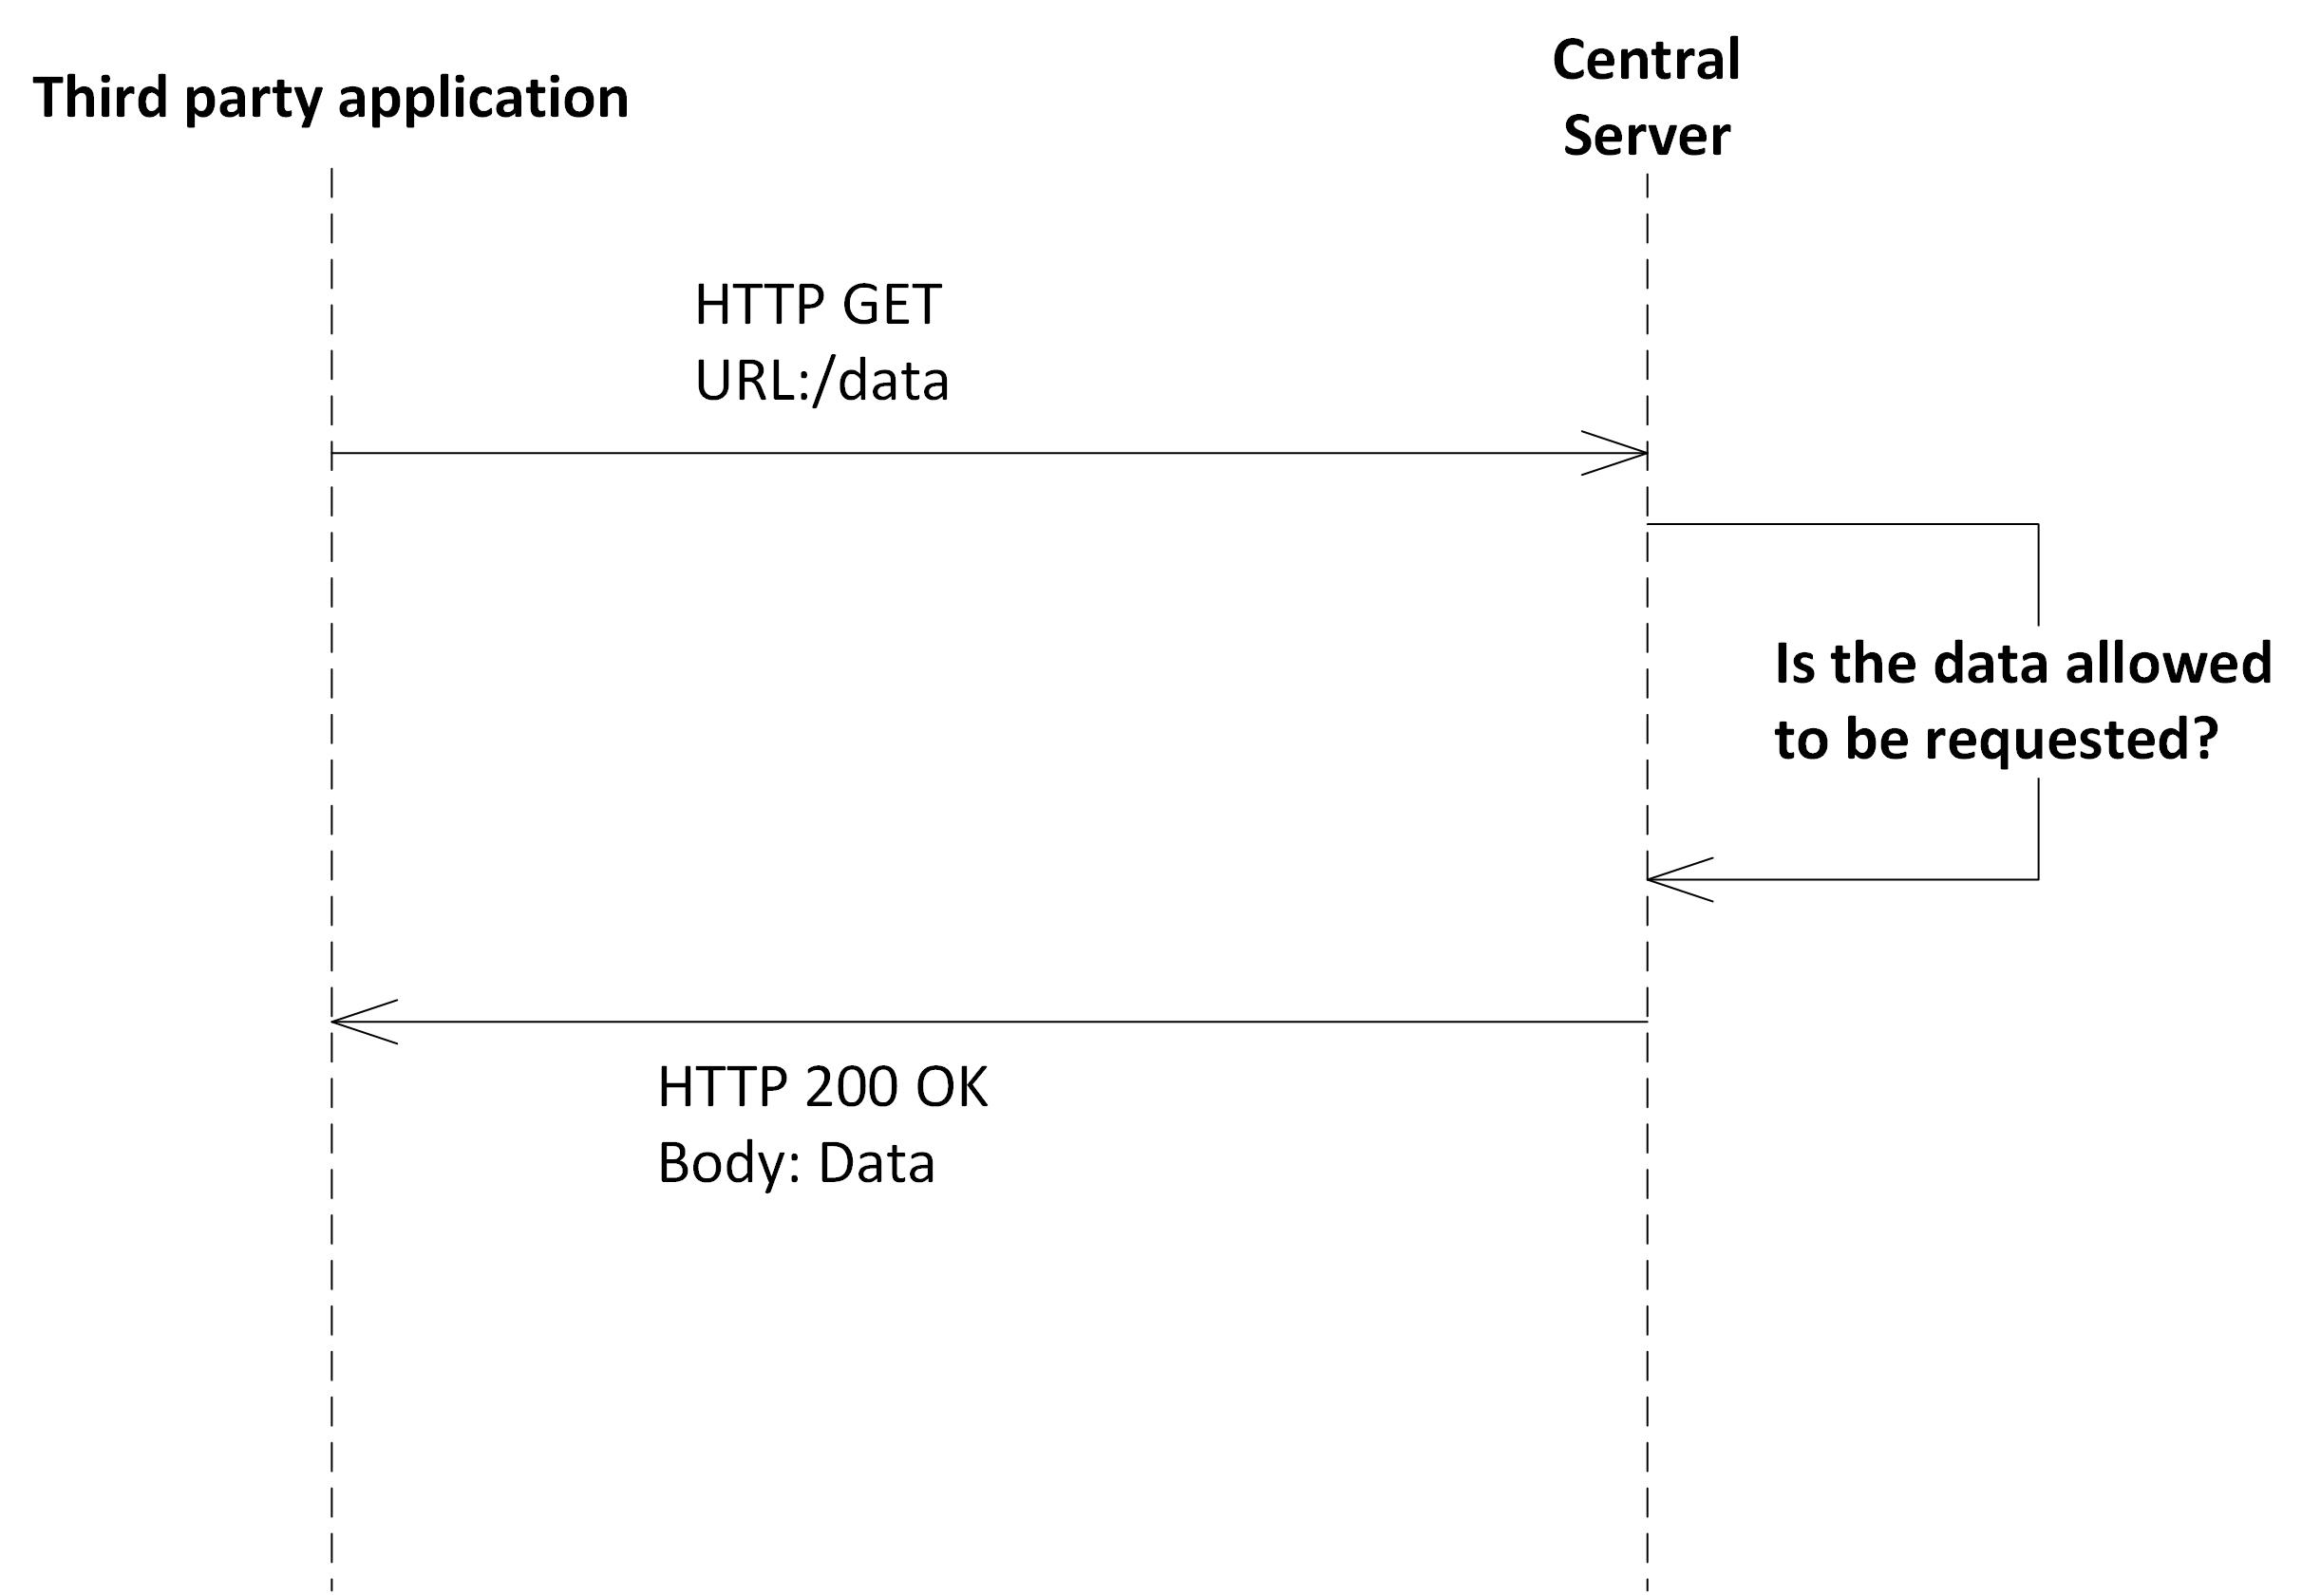
\includegraphics[keepaspectratio=true,width=0.9\textwidth]{{\viewimages/sequencethirdparty}.jpg}
	\caption{Sequence diagram of the client pushing the sensor data}
	\label{fig:thirdpartyseq}
\end{figure}

The API calls the service layer receives that request information, don't need to be authenticated. These calls, however, do need to be limited by the service layer to not be able to delete or modify information. The information the API provides is defined in the server layer and the API does not return any information other then that.\\
The third party sends a http GET request to the REST server of SMF. Upon receiving this request, the REST server checks if the request is secure. This logic is located in the service layer. When the request is secure, the REST server calls the mapper object in order to get the requested data. The mapper object first checks the identity map if the data is already loaded. This will reduce the amount of queries executed on the database. If this identity map doesn't hold the data, the mapper sends a query to the database. The data returned from the database is then returned to the REST server, who sends the data to the third party.

\paragraph{Distribute warnings}
In figure~\ref{fig:warning} a sequence diagram of sending warnings to the emergency room and citizens can be seen. The sequence diagram contains a time constraint of 10 seconds and 5 minutes, for warning the emergency room and all citizens respectively.

\begin{figure}[H]
	\centering
	\includegraphics[keepaspectratio=true,width=1.0\textwidth]{{\viewimages/sequence_warning}.png}
	\caption{A sequence diagram of sending warnings to citizens and emergency room}
	\label{fig:warning}
\end{figure}

%							Downside: Data will be received that was not requested, even if not interested. 
%Three principal layers (p20 poeaa)

\subsubsection*{Domain layer}
The domain layer contains all the logic of the system. This includes the logic for the algorithms used to decide if a warning should be issued. And it includes the logic for managing the sensor data.\\
The sensor manager checks if the sensor is still working correctly.%todo
If the sensor is working correctly, the sensor data gets stored and processed.\\
The class diagram for handling incoming REST server calls is shown in figure \ref{fig:domain1}.
\begin{figure}[H]
	\centering
	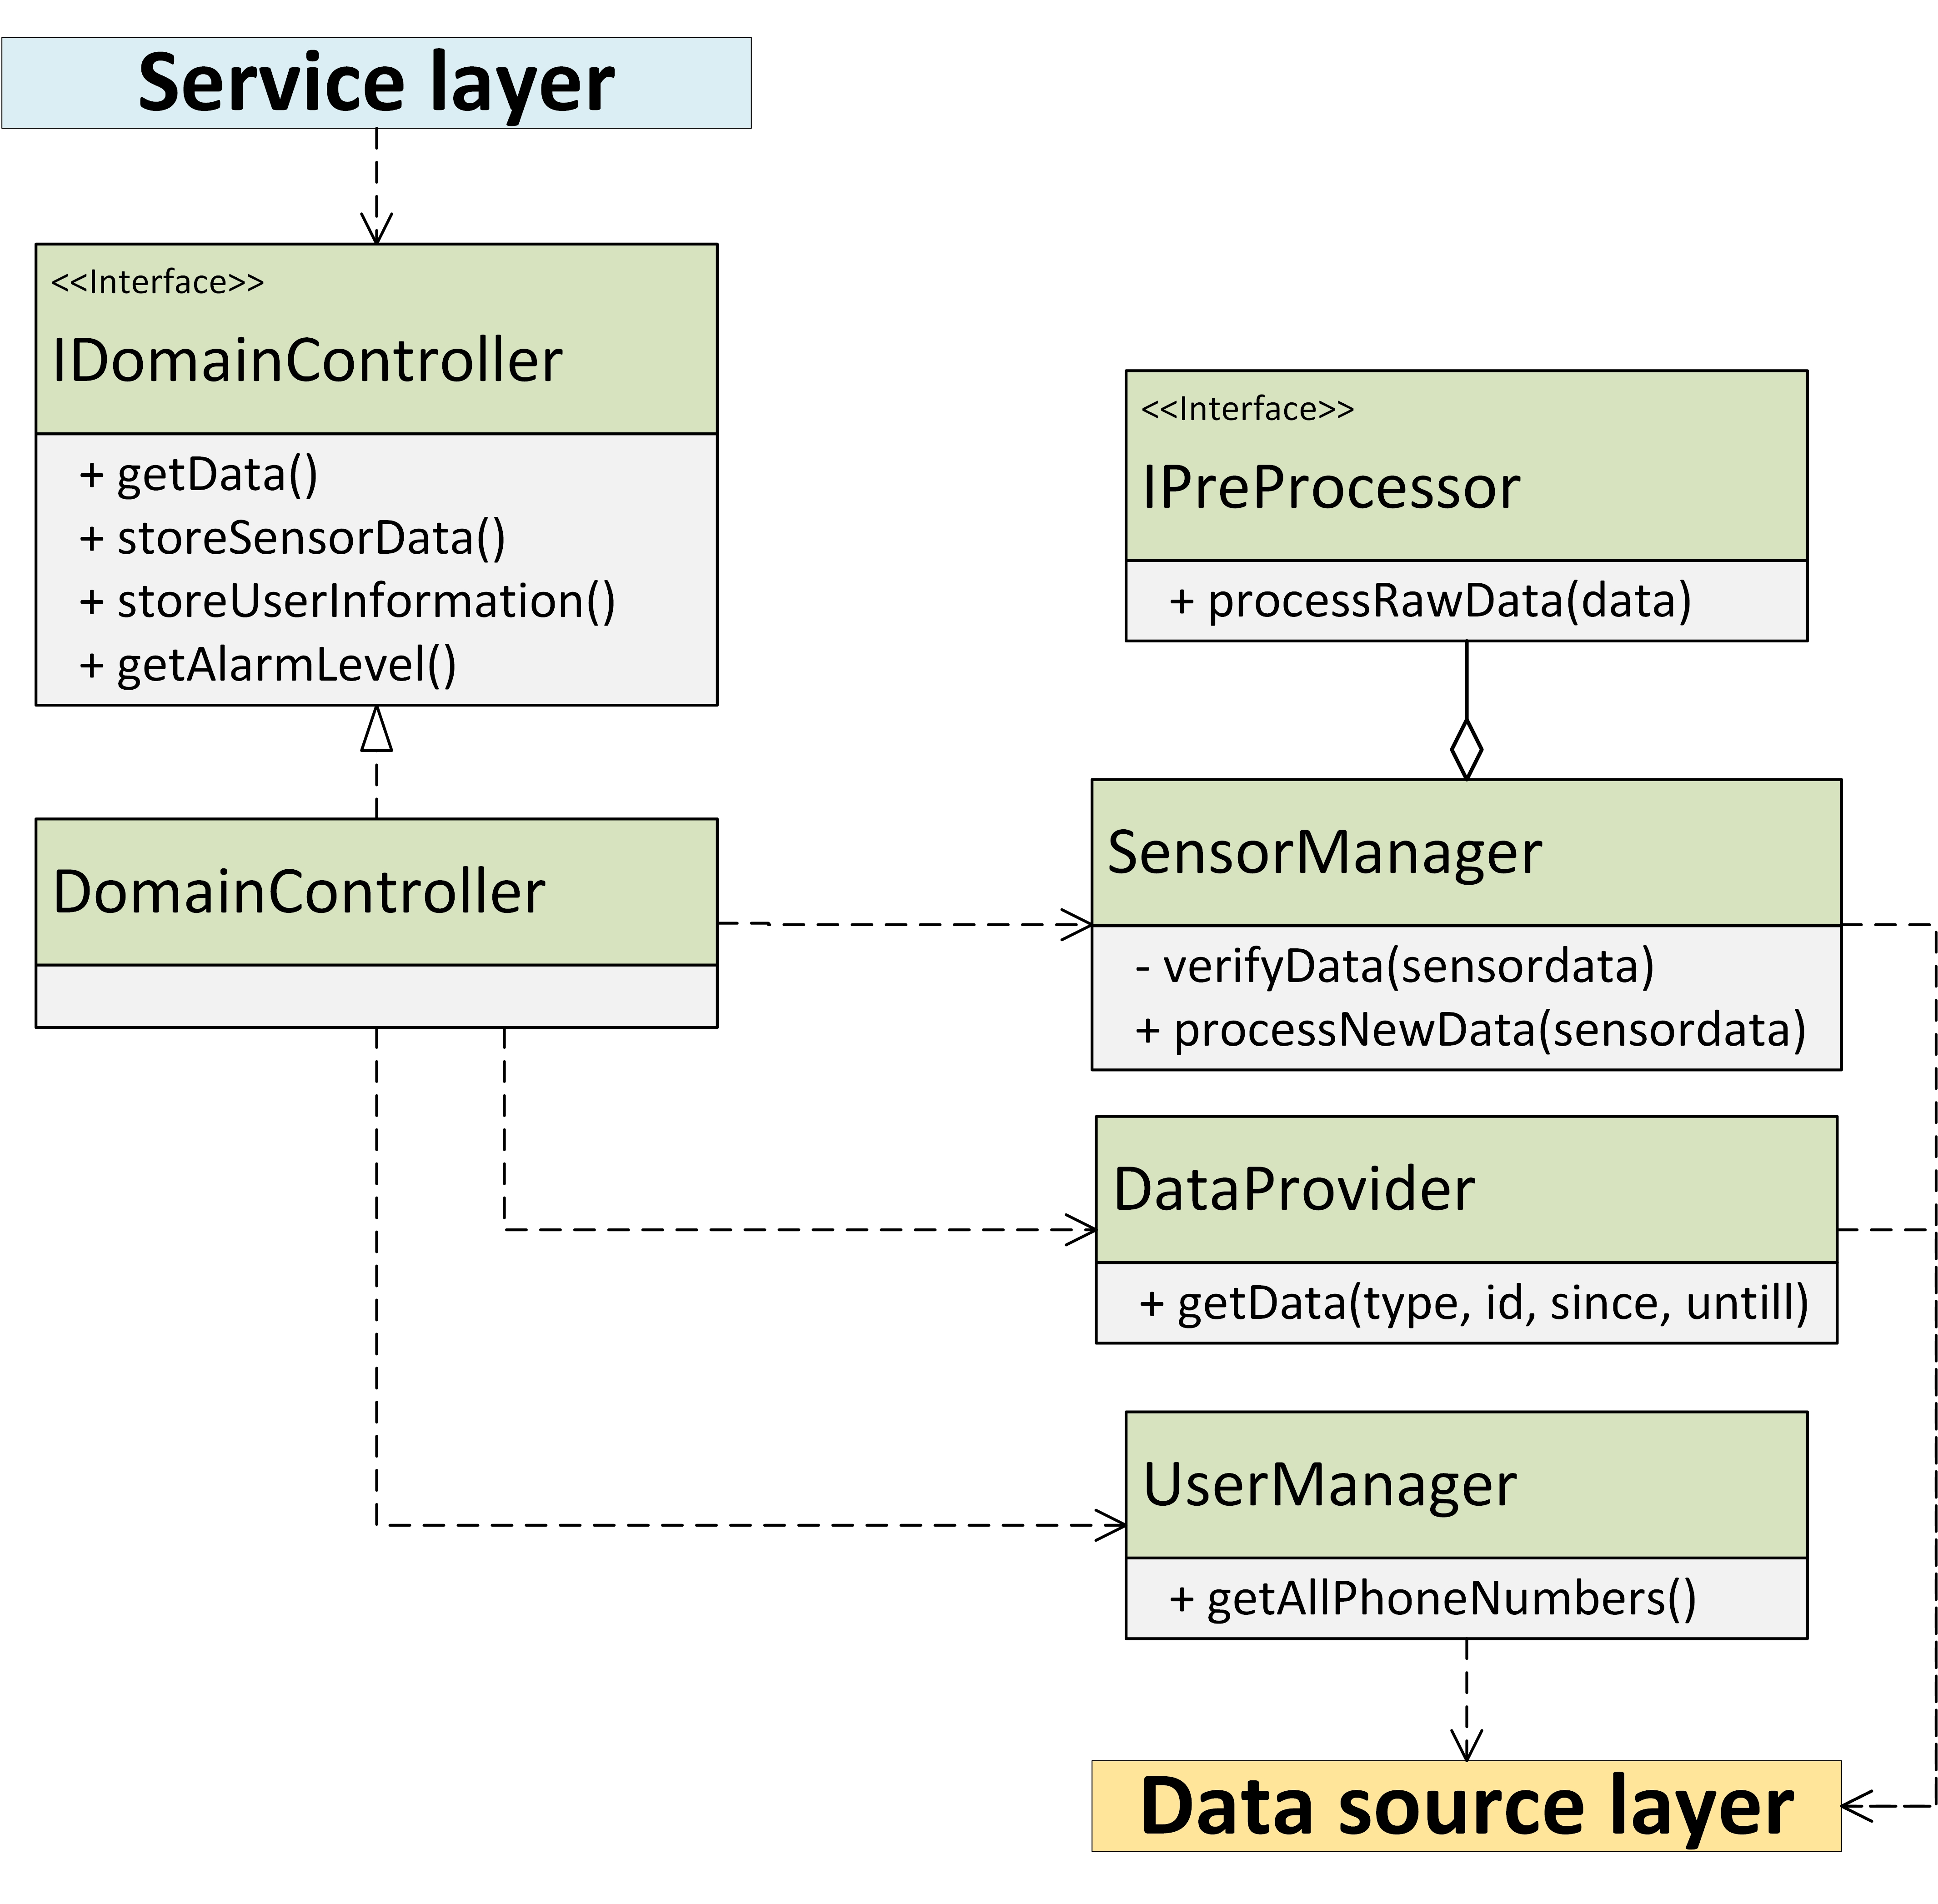
\includegraphics[keepaspectratio=true,width=1.0\textwidth]{{\viewimages/domain1}.jpg}
	\caption{Class diagram of the domain layer concerning REST calls}
	\label{fig:domain1}
\end{figure}

The classdiagramm of the algorithm processing the data is shown below in figure \ref{fig:domain2}

\begin{figure}[H]
	\centering
	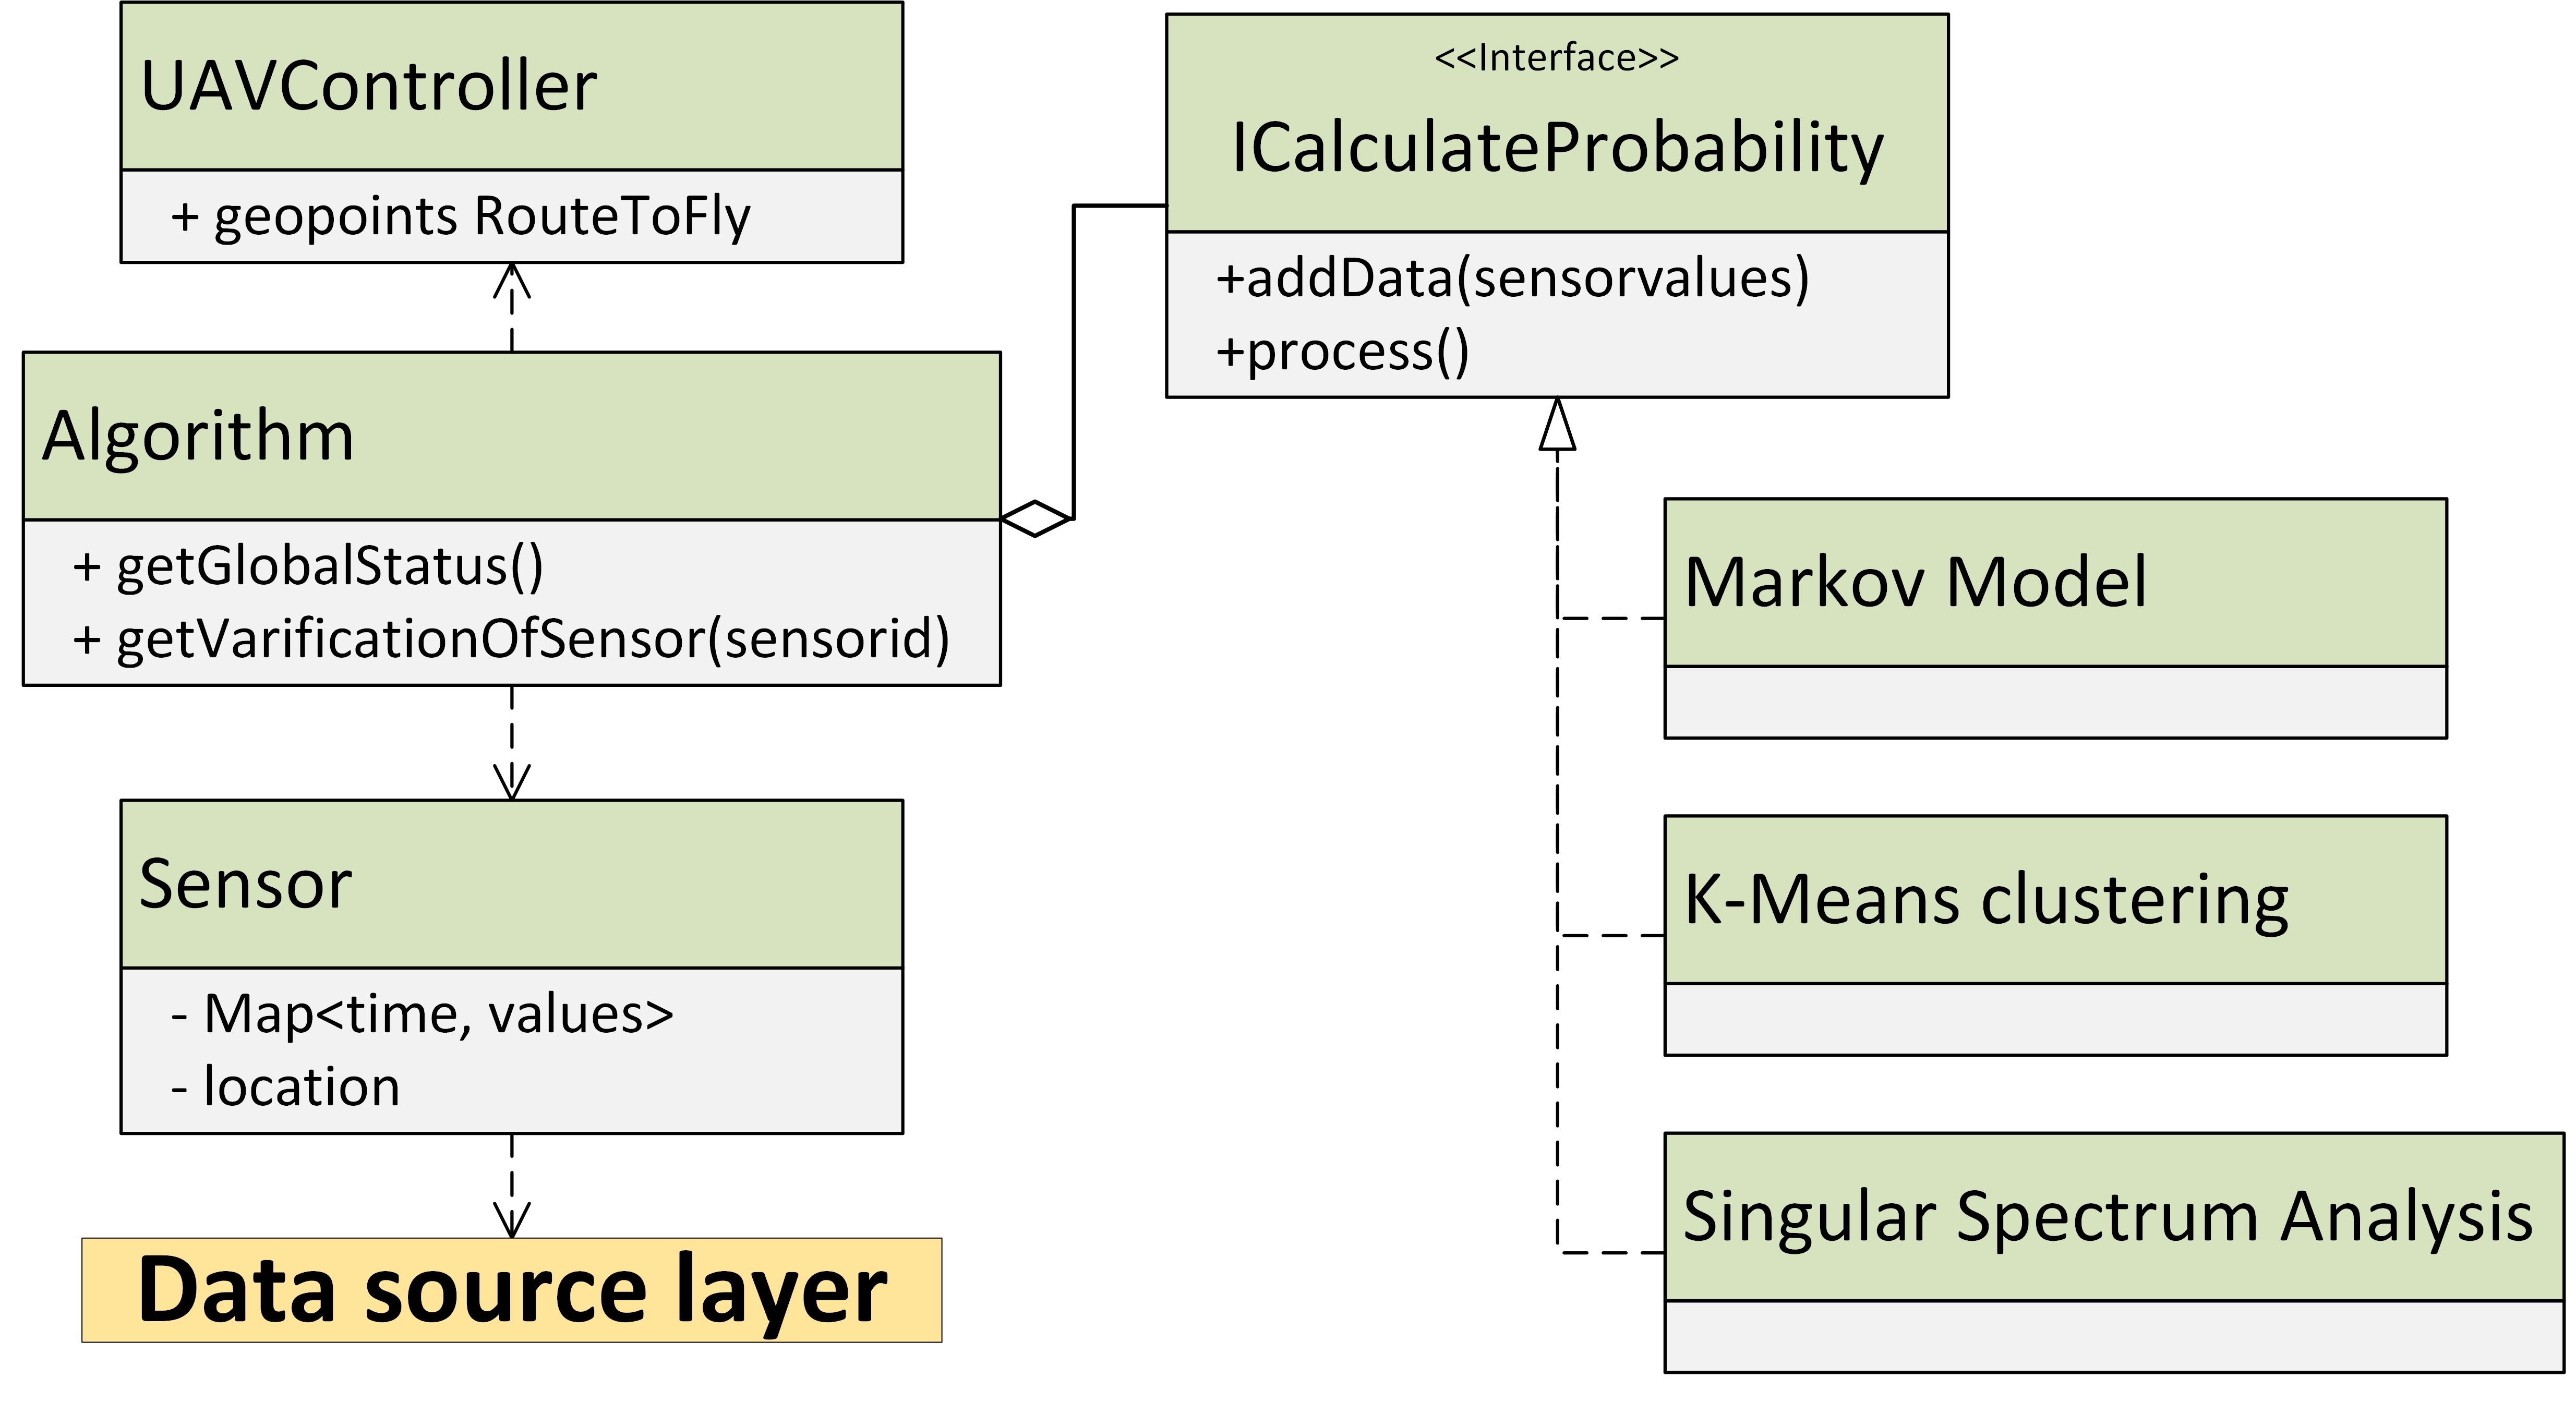
\includegraphics[keepaspectratio=true,width=1.0\textwidth]{{\viewimages/domain2}.jpg}
	\caption{Class diagram of flood prediction in the domain layer}
	\label{fig:domain2}
\end{figure}
First the incoming sensor data is getting pre processed. 
This is done by using:
\begin{itemize}
	\item Smoothing the L1 norm using the Huber function 
	\item Hodrick–Prescott filter
\end{itemize}

The the L1 norm smoothing fluctuates more than the Hodrick-Prescott function. This way, the long term and short term differences can be analyzed better.\\

%https://en.wikipedia.org/wiki/Hodrick%E2%80%93Prescott_filter
%http://mathoverflow.net/questions/118333/smoothing-l1-norm-huber-vs-conjugate
%
After the pre processing, the sensor data gets stored and will be used in several algorithms to calculate a flood probability.
There are several algorithms being used, these are:
\begin{itemize}
	\item Hidden Markov model with k-means clustering
	\item Singular Spectrum Analysis (SSA) for locations with tides
	\item Limit checking
\end{itemize}

Limit checking is just checking if the value of the sensor is not above a certain limit. A sudden extreme value will be detected using limit checking. If there are more sensors giving extreme values, the domain layer will verify this sudden change and might then issue the service layer to send a warning message.\\
SSA splits the range of values into blocks and then checks for abnormalities within that block.\\
The k-means clustering algorithm is used to detect abnormalities in the sensor data coming from a certain range dike. This way all the sensors should measure about the same values. In order to check for abnormalities, the k-means clustering can detect when a sensor value is out of the cluster.\\

%corrdata slide 60
How strongly correlated two types of data are will be calculated using Longitudinal Data Analysis.

\subsubsection*{Data source layer}
The data mapper \cite{Fowler:2002:PEA:579257} is used to completely separate and ignore the database in the domain model. The domain object only uses an interface to a "find" function that returns the requested object. This could be either from the database or from the internal memory.\\
How the database is structured will be discussed in the implementation view section.

% \begin{figure}[H]
% %\centering
% 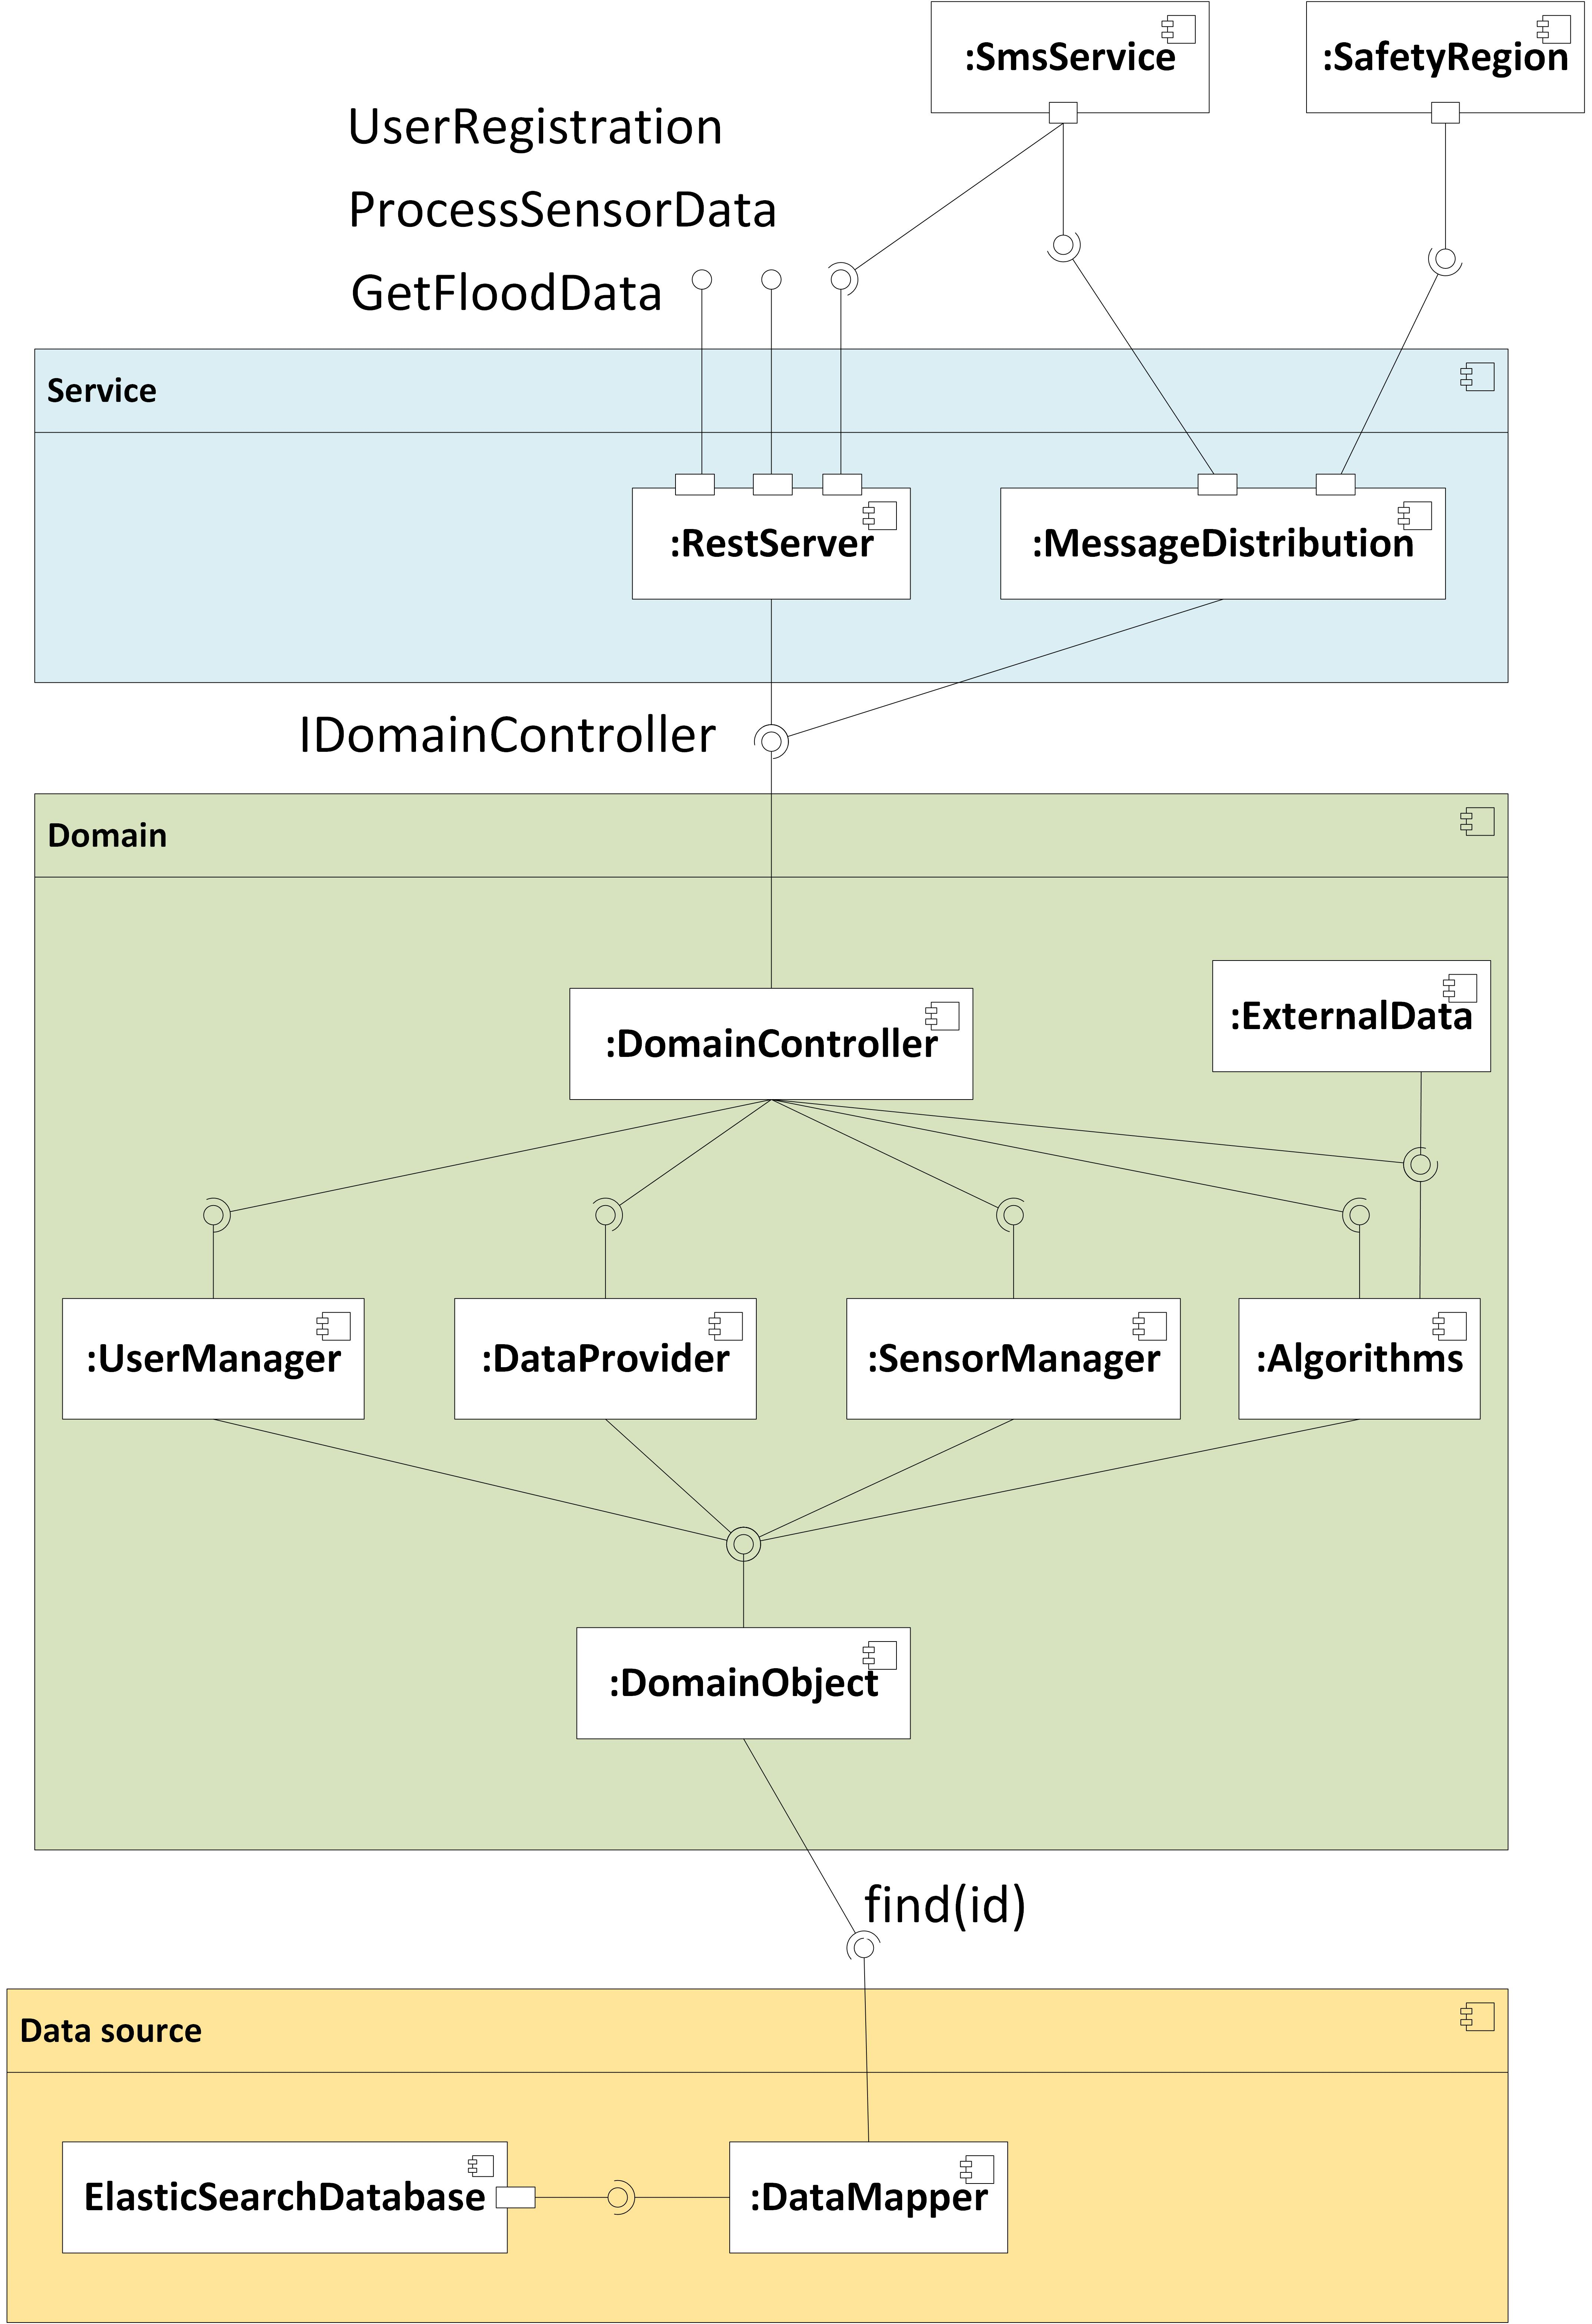
\includegraphics[keepaspectratio=true,width=0.9\textwidth]{{\viewimages/component}.jpg}
% \caption{Component diagram}
% \label{fig:component}
% \end{figure}



% \clearpage
% \begin{figure}[H]
% %\centering
% 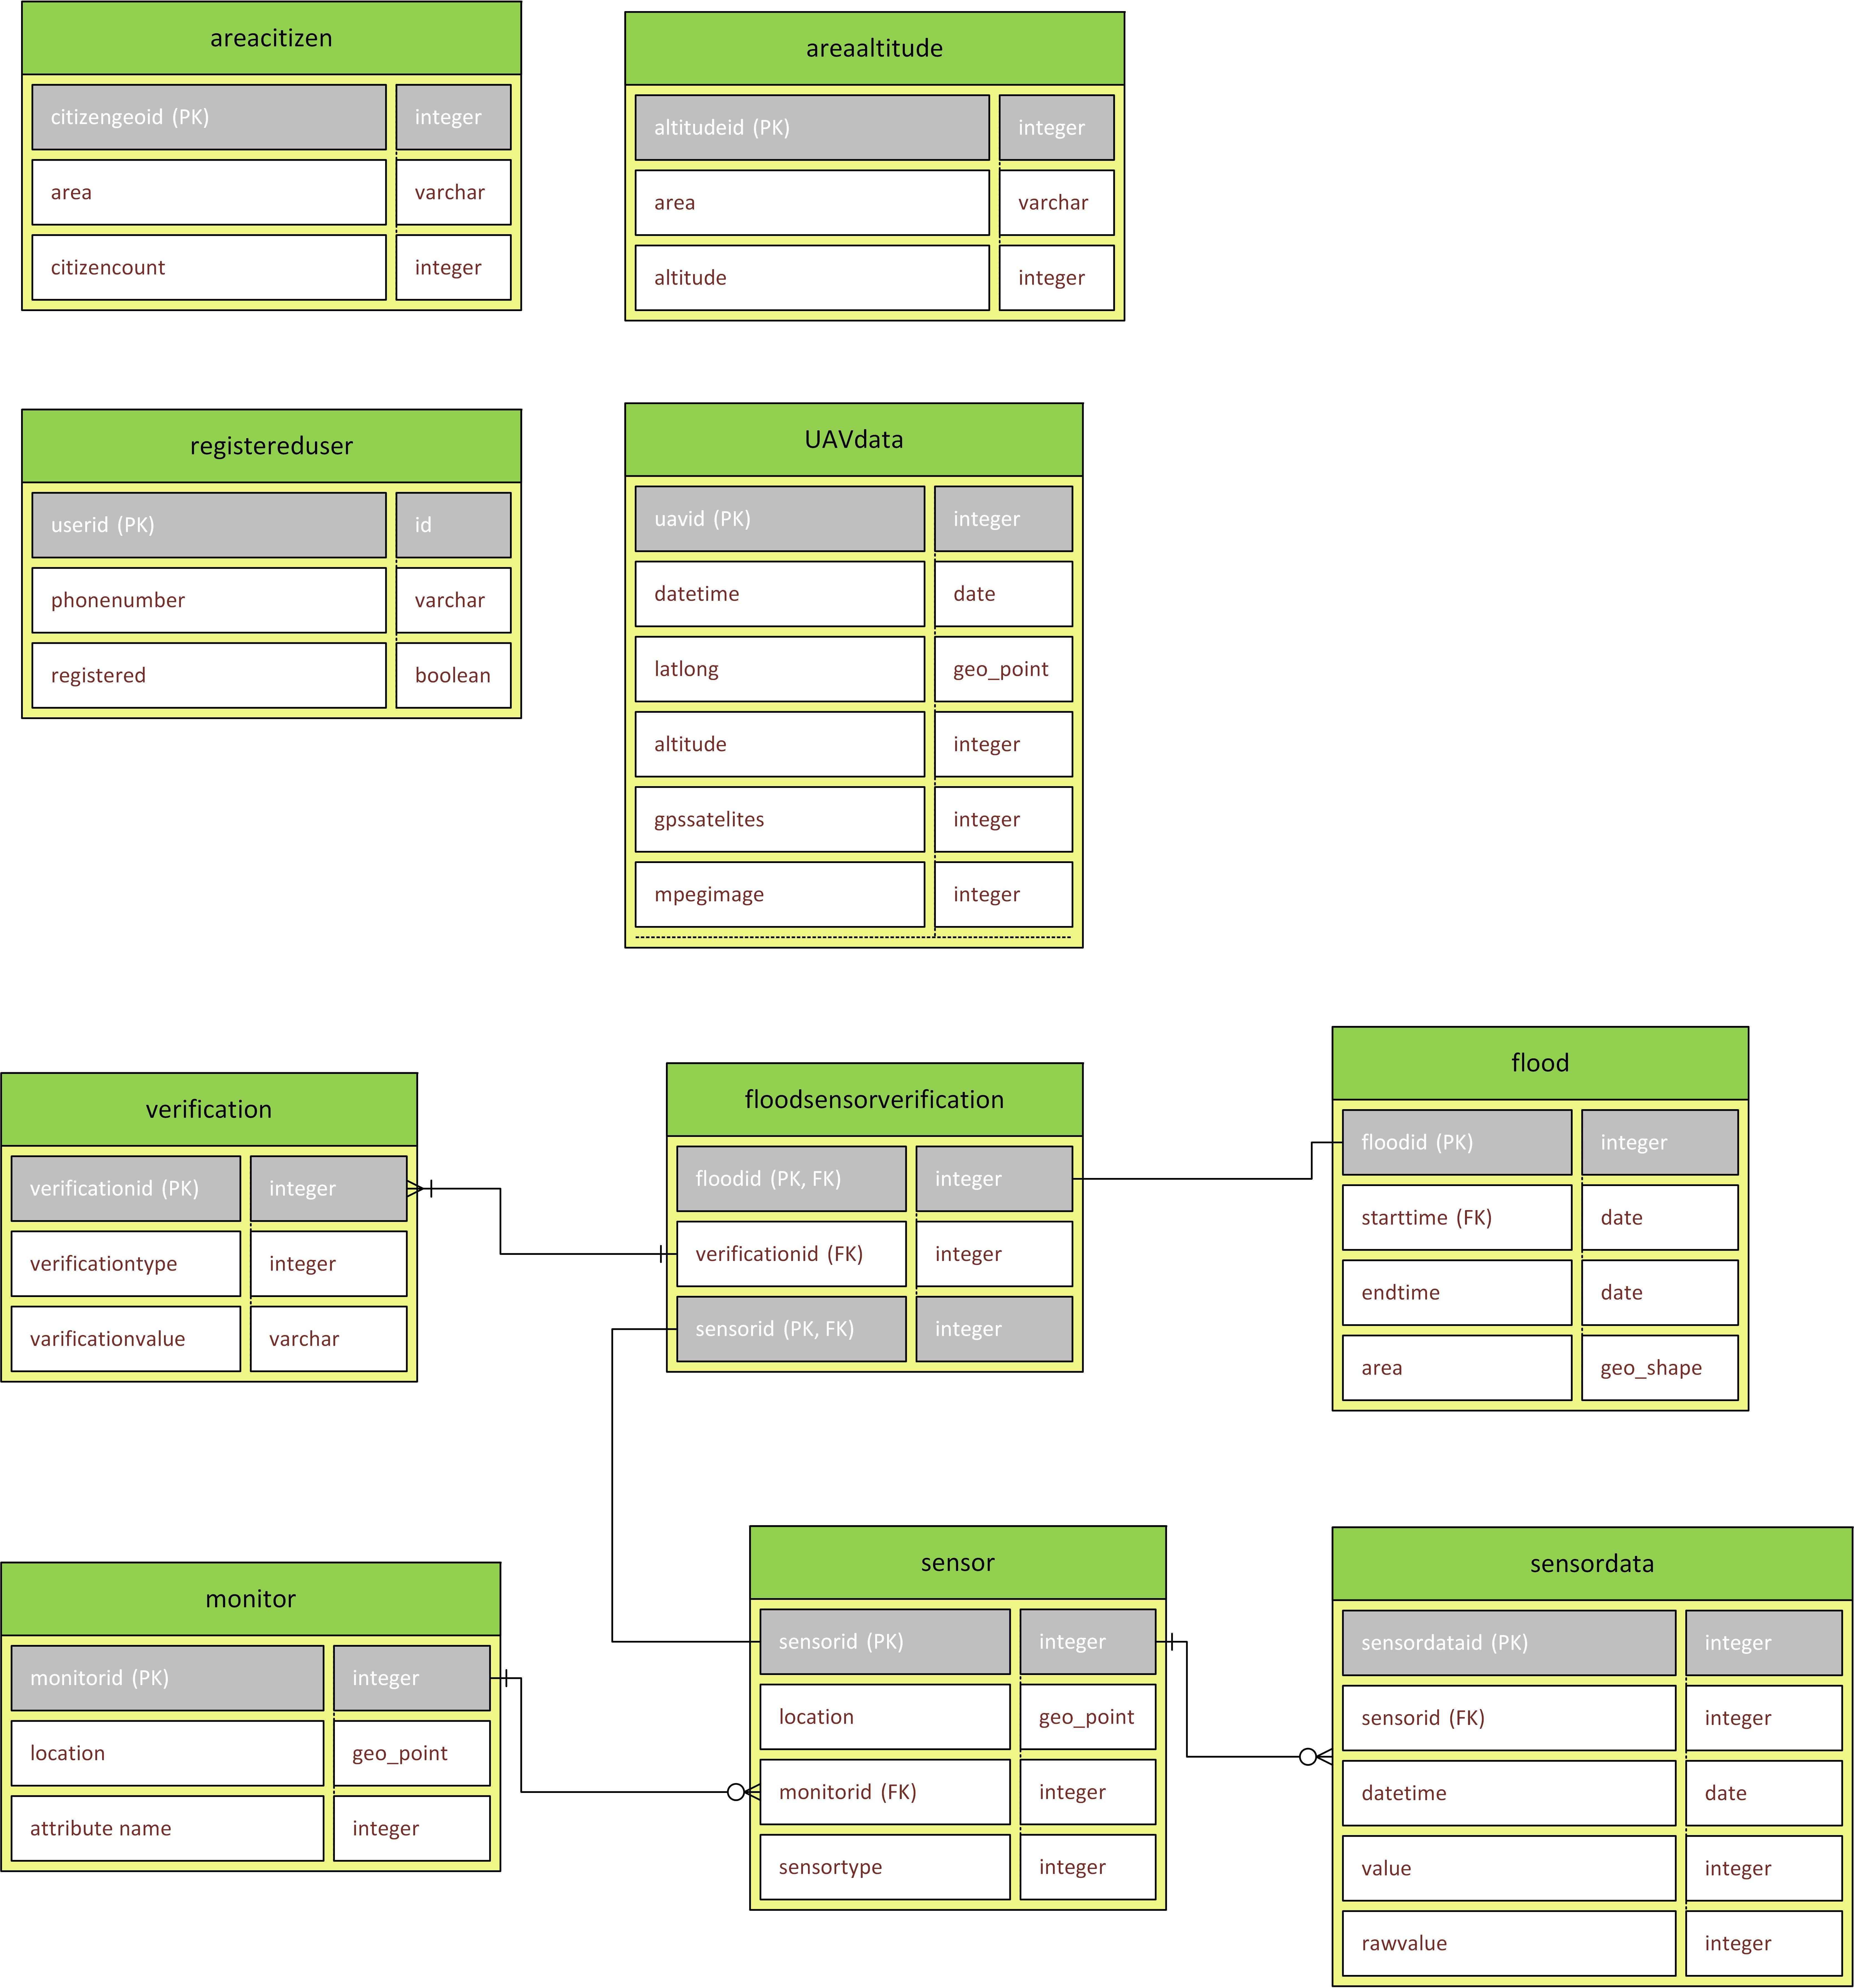
\includegraphics[keepaspectratio=true,width=0.9\textwidth]{{\viewimages/database}.jpg}
% \caption{Database diagram}
% \label{fig:component}
% \end{figure}

% \begin{figure}[H]
% %\centering
% 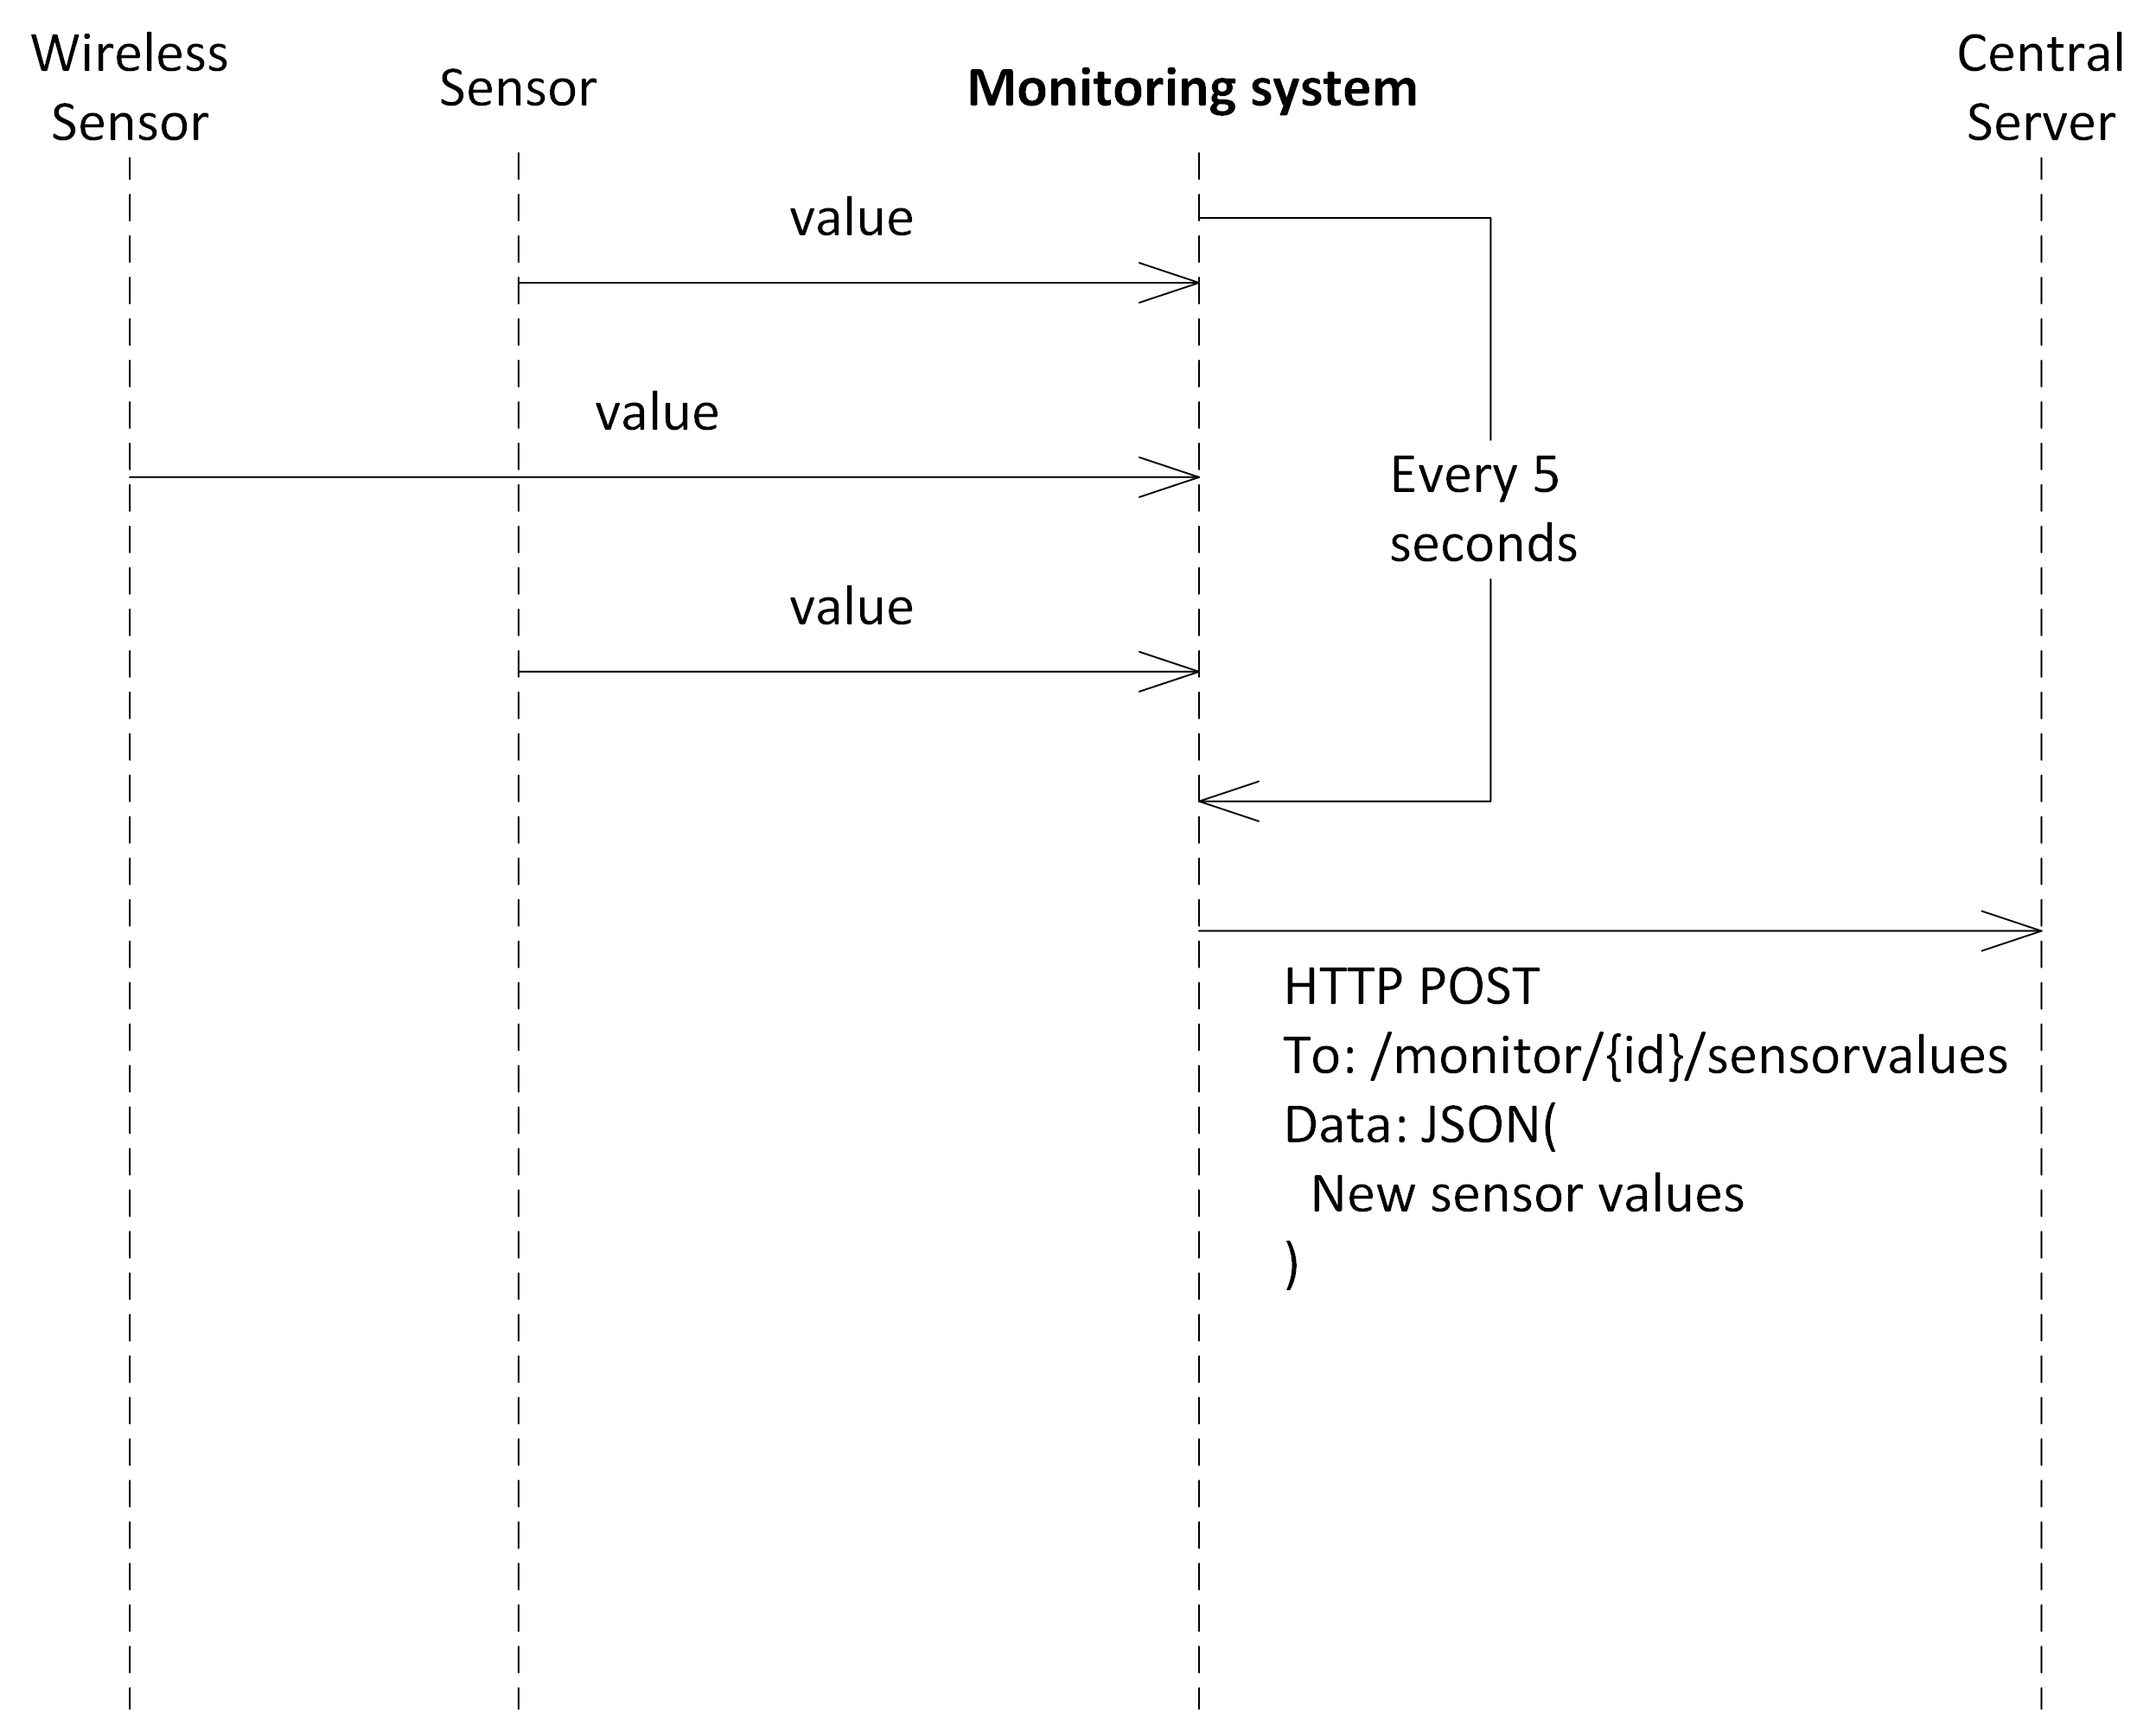
\includegraphics[keepaspectratio=true,width=0.9\textwidth]{{\viewimages/sequence1}.jpg}
% \caption{Sequence diagram of the client pushing the sensor data}
% \label{fig:component}
% \end{figure}
%\begin{framed}
%
%	Update monitor system firmware? Do we do this? And how do we do this?
%	Do sensors have firmware and how do we update that?
%
%\end{framed}

